\documentclass[10pt, a4paper]{aqademic}

\usepackage[spanish]{babel}
	\selectlanguage{spanish}

% Document packages

\usepackage[type=CC, modifier=by-nc-sa, version=4.0]{doclicense}
\usepackage{graphicx}
	\graphicspath{{img}}
\usepackage{hyperref}
\usepackage{url}

% Custom commands

\def\mysim{\raise.17ex\hbox{$\scriptstyle\mathtt{\sim}$}}

% Document settings

\author{Atanasio José Rubio Gil}
\title{Neosluger}

% Document composition

\begin{document}

\AqMaketitle[%
	author   = Atanasio José Rubio Gil,
	cover    = logo-ugr.png,
	org      = Oficina de Software Libre,
	subtitle = Manual de usuario,
	url      = https://github.com/OSL-UGR/neosluger
]
\tableofcontents

\chapter{El servicio}\label{el-servicio}

\section{¿Qué es Neosluger?}\label{que-es-neosluger}

Neosluger\footnote{
	\url{https://github.com/OSL-UGR/neosluger}
} es una reescritura completa de Sluger\footnote{
	\url{https://github.com/OSL-UGR/sluger}
},
el acortador de enlaces de la Universidad de Granada cuyo nombre significa \textbf{S}hort \textbf{L}ink \textbf{UGR} (se añade una \textit{e} para ayudar a la pronunciación).
Neosluger es Software Libre, lo que significa que eres libre de modificarlo y distribuirlo siempre y cuando te atengas a las condiciones y obligaciones impuestas por su licencia.

La versión antigua ofrecía un acortador de enlaces, una API y estadísticas de uso públicas para cada enlace corto.
Esta versión renueva la API y ofrece un generador de códigos QR que puede ser usado libremente para cualquier enlace, no sólo para los acortados.
Al igual que en la versión antigua, el acortador de enlaces está disponible únicamente para usuarios que accedan al servicio desde la red de la UGR, pero el resto de servicios están disponibles para el público general.
Esto nos asegura que todos los enlaces sean creados para propósitos relacionados con la UGR.

El servicio nuevo se encuentra disponible en la misma dirección que el original: \url{https://sl.ugr.es/}

\section{La interfaz web}\label{la-interfaz-web}

\begin{figure}[ht!]
	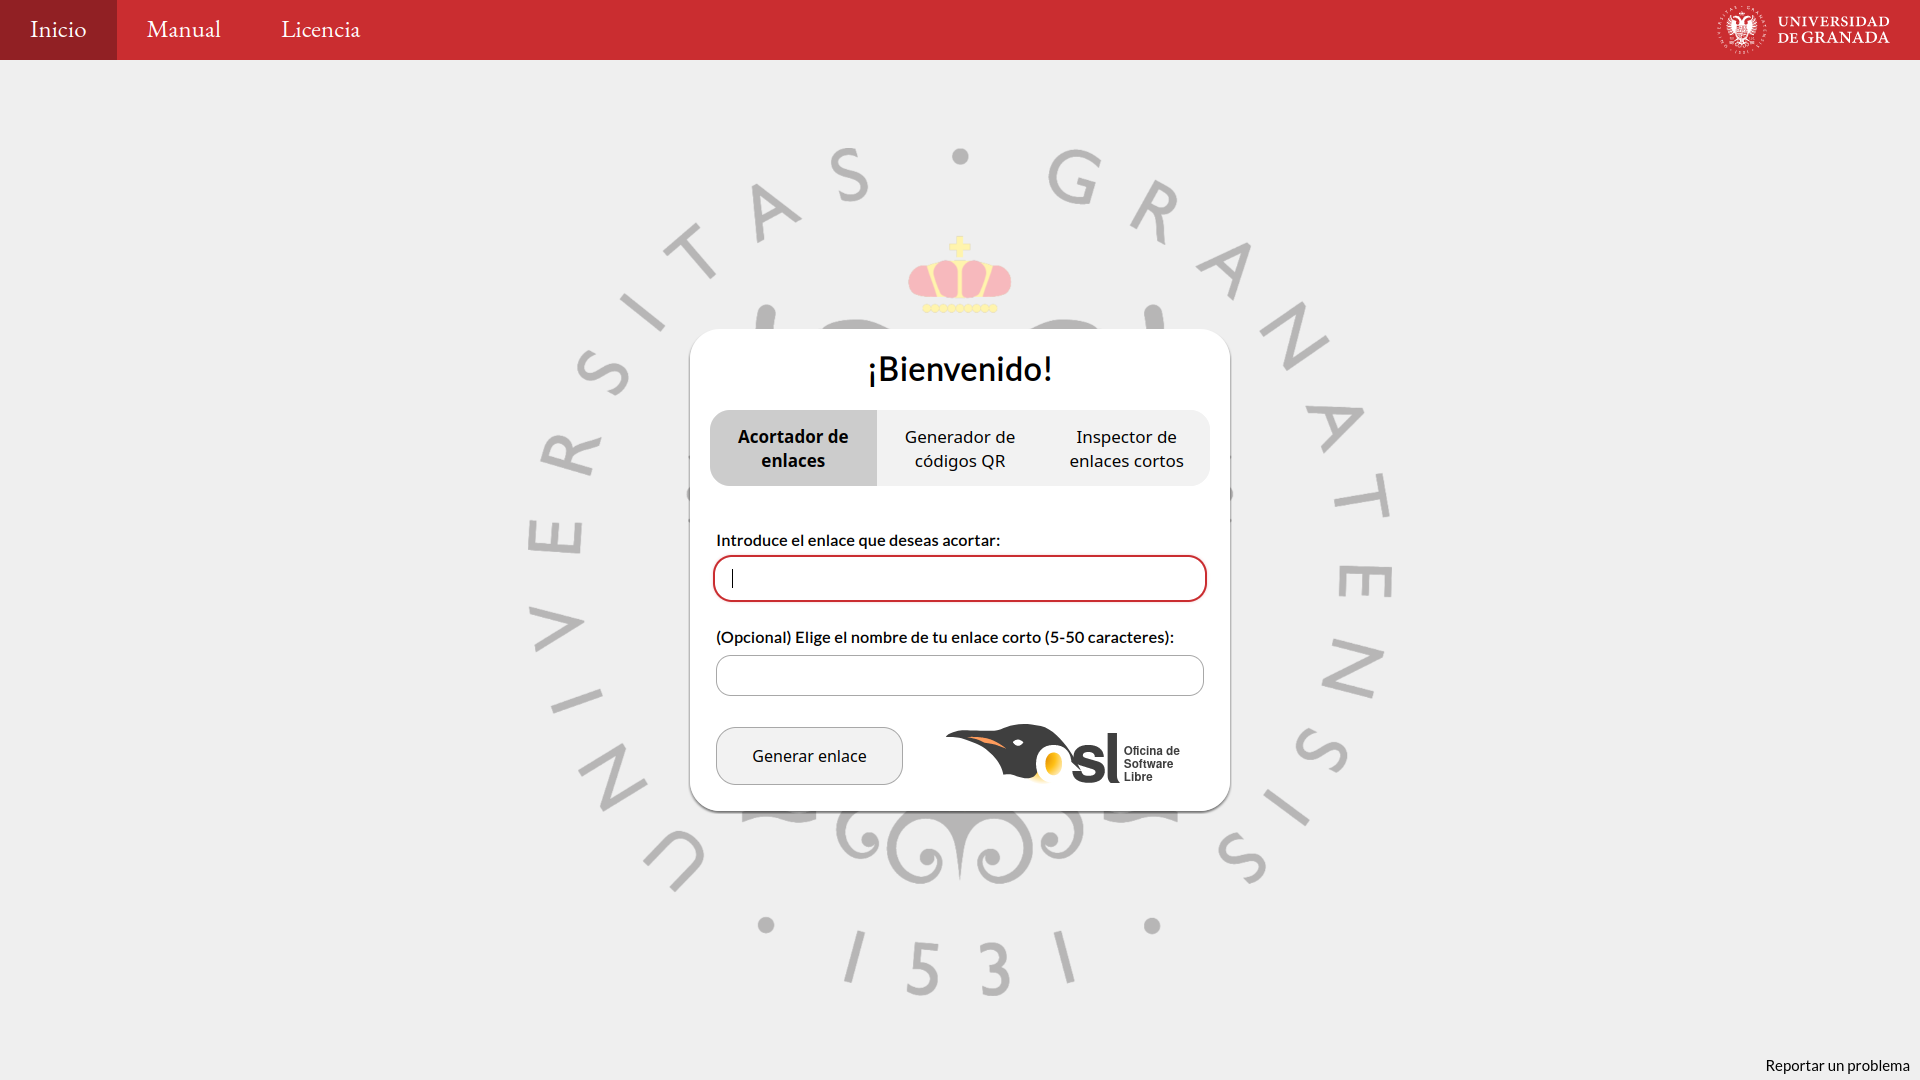
\includegraphics{web-index}
	\caption{La página de inicio de Neosluger.}
\end{figure}

La interfaz web de Neoswluger está dividida en tres pestañas:
La pestaña de \textit{Inicio} es la primera que ve el usuario y contiene el \textit{acortador de enlaces}, el \textit{generador de códigos QR} y el \textit{inspector de enlaces cortos}.

La pestaña del \textit{Manual} contiene instrucciones de uso para el acortador de enlaces, el generador de códigos QR y la API.
La pestaña de \textit{Licencia} contiene la licencia del servicio, un enlace al texto original de GNU, una versión en bruto de la licencia y un enlace al repositorio de Neosluger.
Cada página contiene un botón para \textit{Reportar un problema} que al usuario a una página en la que pueden contactar con la Oficina de Software Libre de la UGR para modificar o eliminar un enlace o para que arreglen un error lo antes posible.

\begin{figure}[ht!]
	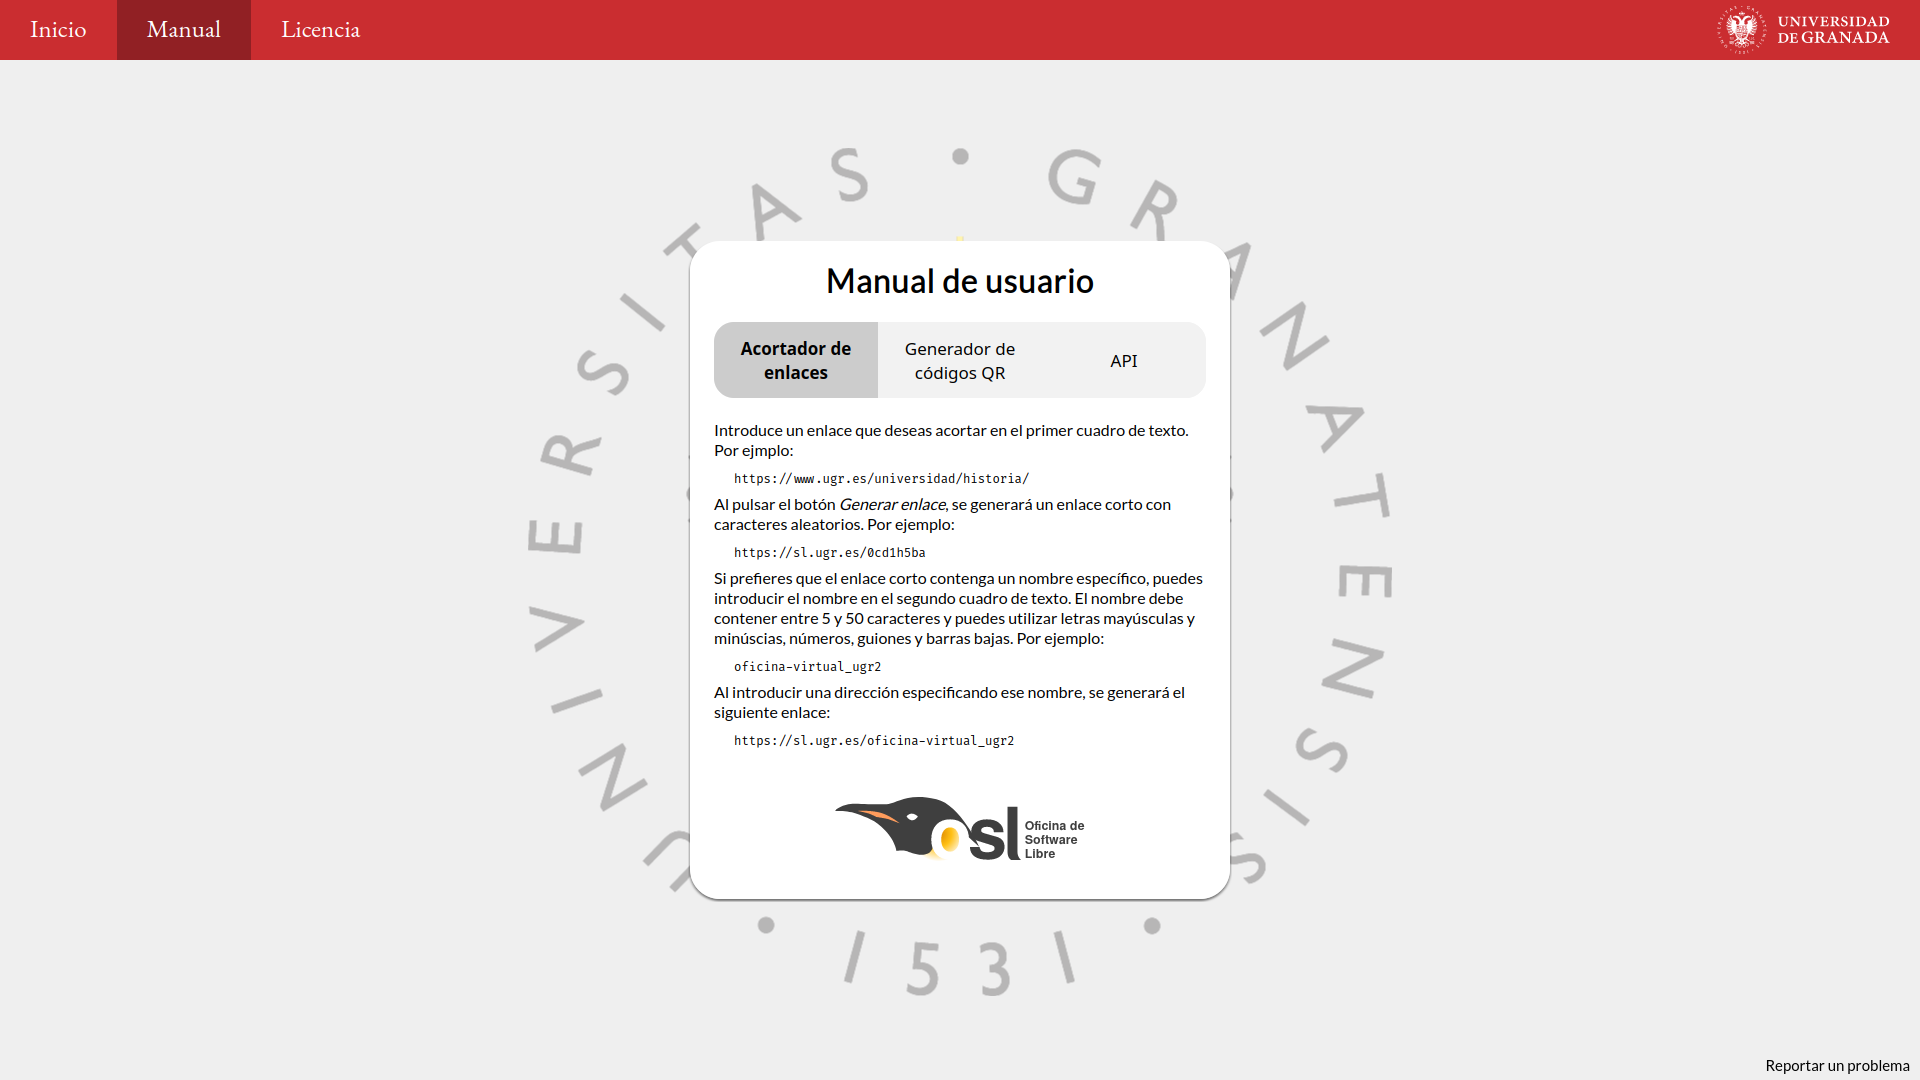
\includegraphics{web-man}
	\caption{La página del manual de Neosluger.}
\end{figure}

\begin{figure}[ht!]
	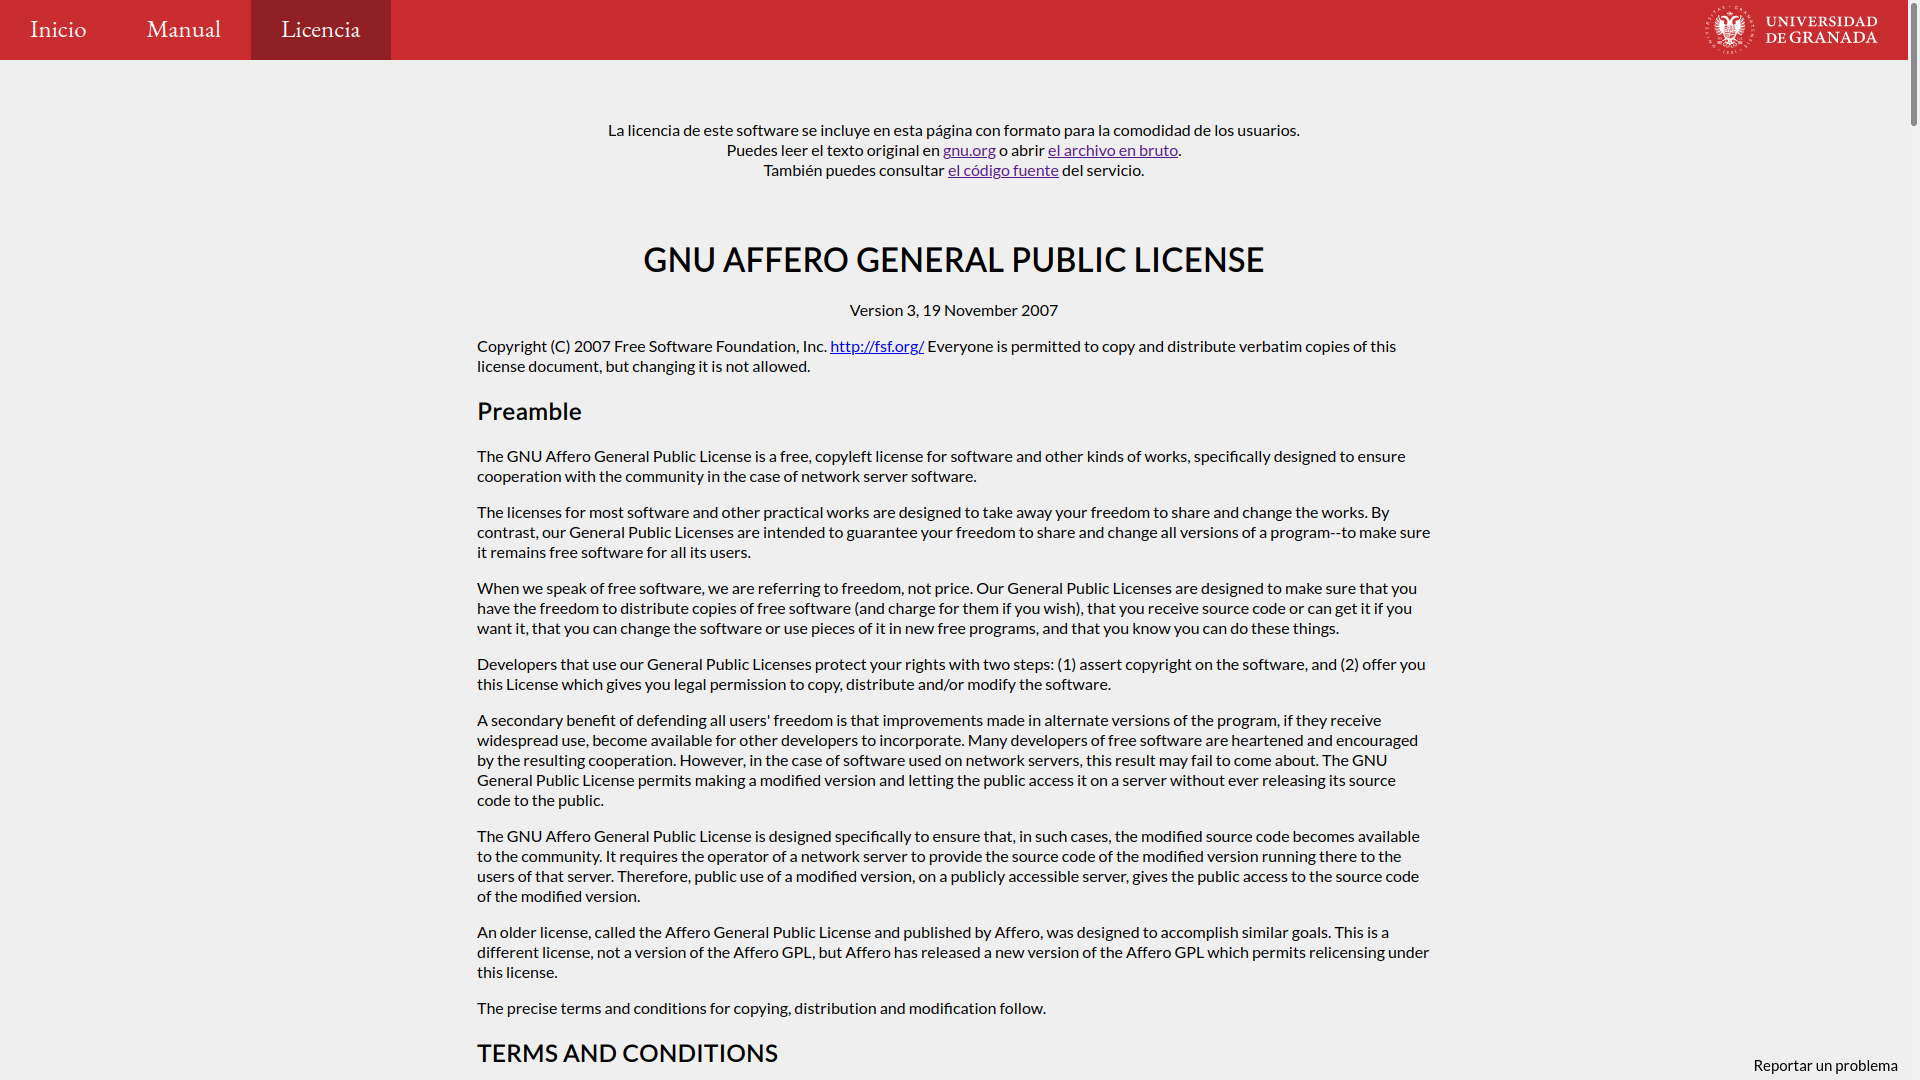
\includegraphics{web-licence}
	\caption{La página de la licencia de Neosluger.}
\end{figure}


\section{La API}\label{la-api}

Otra forma de acceder al servicio es mediante su API (\textit{Application Programming Interface}), que permite a otros programas interactuar con él sin tener que usar la interfaz web.
Su uso se detallará en su propia sección.

\begin{figure}[ht!]
	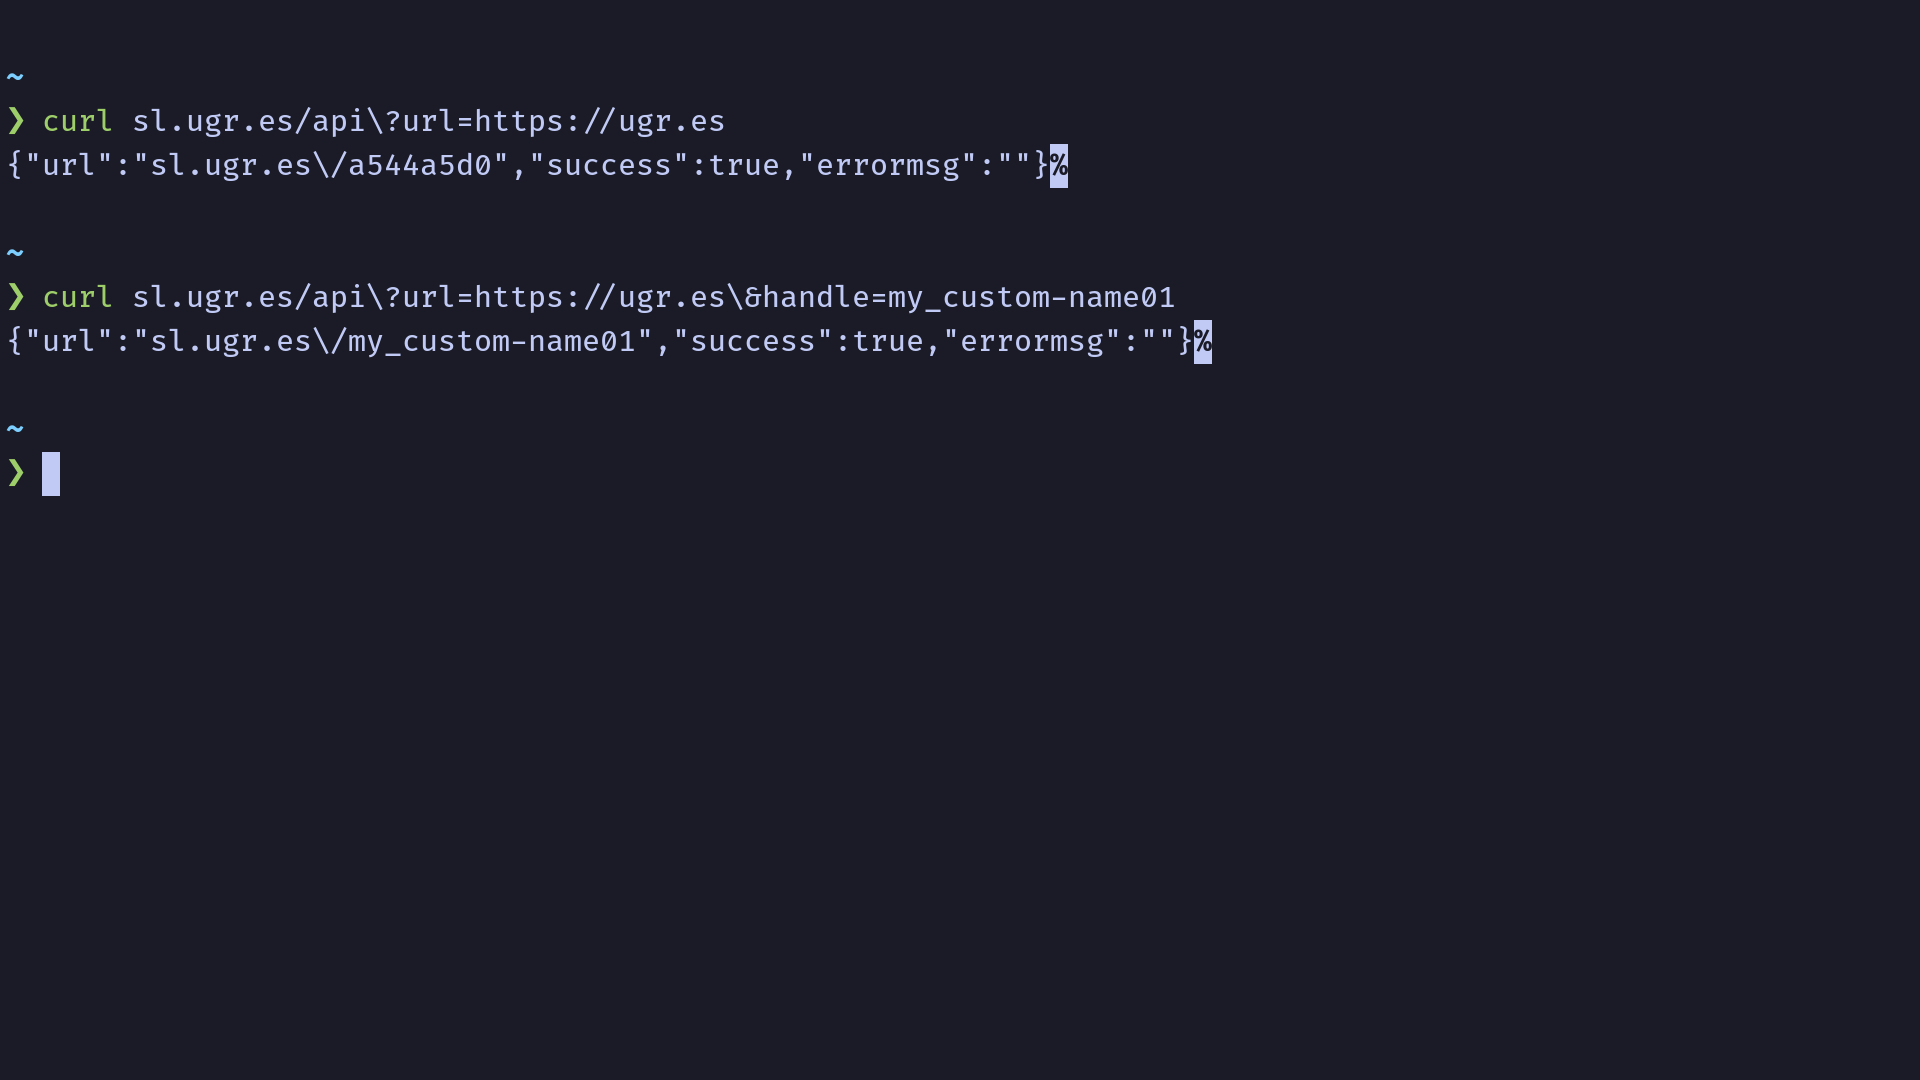
\includegraphics{api-curl}
	\caption{Enlaces cortos creados con la API.}
\end{figure}

\input{input-es/Configuración del servidor}
\input{input-es/Resolución de enlaces}

\end{document}
